
\documentclass[twoside]{protokoll}
\usepackage{graphicx}
\praktikum{I}

\versuchsgebiet{(Akustik)}


\teilnehmer{Maximilian Carlos Menke, 434170}
\teilnehmer{Andrea Roth, 428396}
\gruppe{A3}

\begin{document}

\begin{versuchsziele}
Ziel des Versuches ist, das Elastizitätzsmodul verschiedener Metallstäbe zu bestimmen.
Eine statische Messung liefert nur für dünne Drähte Ergebnisse weswegen das Elastizitätsmodul in unserem Fall mit einer Dynamischen Messung bestimmt wird. Hierfür erzeugen wir stehende Wellen in den Metallstäben. So können wir mit der Frequenz und der Wellenlänge die Phasengeschwindigkeit und somit auch das Elastizitätsmodul bestimmen. 
\end{versuchsziele}

 
\section{1A3 Bestimmung des E-Moduls von Metallen}

\begin{aufgabe}{Grundlagen}
  % Knappe Beschreibung der theoretischen Grundlagen, Angabe der
  % Fbenötigten Formel(n), ohne Herleitung. Definition der verwendeten
  % Formelzeichen.
    Da wir keine Statische Messung des E-Moduls durchführen können, verwenden wir hier eine dynamische Messung.
    Für diese brauchen wir Wissen aus der Akustik über stehende Wellen, als auch von Festkoerpern.


    Das E-Modul ist ein Maß für die Dehnbarkeit eines Materials. Es ist Definiert als: 
    \begin{equation}
        E = \frac{\frac{F}{A}}{\frac{\Delta L}{L}}
    \end{equation}


    Wenn der Stab in Schwingung versetzt wird, bliden sich stehende Wellen in ihm aus.
    Wir wollen hierbei die Frequenz der Grundschwingung bestimmen.
    Da der Stab an beiden Enden ein festes Ende für die Wellen hat, muss für Resonanz der Grundschwingung die Wellenlaenge: $\lambda = 2 * L$. 
     
    Daraus ergibt sich:
    \begin{equation}
        v = f * \lambda = f * 2 * L
    \end{equation}

    In Luft breitet sich Schall immer als Longitudinale Welle aus.
    In Festkörpern muss die Rückstellkraft des Materials nicht zwangsweise entgegen der Ausbreitungsrichtung zeigen, weshabl hier allgemein auch eine Transversalve Komponenten vorliegen kann.
    Die Metallstäbe können aber als homogen genung angenommen werden, weshalb wir hier von einer longitudinal Welle ausgehen können.
    Aus der Wellengleichung ergibt:
    \begin{equation}
         v = \sqrt{\frac{E}{p}}
    \end{equation}
    \begin{equation}
         E = v ^2 * p
    \end{equation}
    \begin{equation}
         E = f * \lambda = 4 * f_0 * L ^2 * p
    \end{equation}
    \begin{equation}
        E = f * \lambda = \frac{ 4 * f_0^2 * L ^2 * M}{\pi * (\frac{d}{2}) ^2}
    \end{equation}
    \begin{equation}
        E = f * \lambda = \frac{ 16 * f_0^2 * L ^2 * M}{\pi * d ^2}
    \end{equation}

     
\end{aufgabe}


\begin{aufgabe}{Versuchsaufbau und Versuchsdurchführung}
  Für die Bestimmung des E-Moduls messen wir die Schallwellen die mithilfe eines Gummihammers in dem Stab erzeugt wurden. Diese werden in ein Digitales Signal umgewandelt das wir mithilfe des Sensor CASSY darstellen können und analysieren. Hierzu benötigen wirfolgende Geräte.\\

\textbf{Benötigte Geräte:}
\begin{itemize}
\item Semsor CASSY
\item Universalmikrofon mit Stativstange
\item Sockel
\item Tischklemme
\item Metallstange (Länge: 20cm)
\item Kreuzmuffe
\item Metallstift (Qürschnitt: 4mm, Länge: 30mm)
\item Gummi-Hammer
\item Mikrometerschraube (Messbereich: 0-25mm, Genauigkeit: $\pm$ 0.01mm)
\item Stahl-Bandmaß (Länge: 2m, Tolleranz: $\pm$ 0.7mm)
\item verschiedene Metallstangen (Kupfer, Messing, Stahl, Aluminium)
\item Analysewaage Sartorius BL 1500 (Genauigkeit: $\pm$ 0,2g)
\end{itemize}
\graphicspath{ {./} }
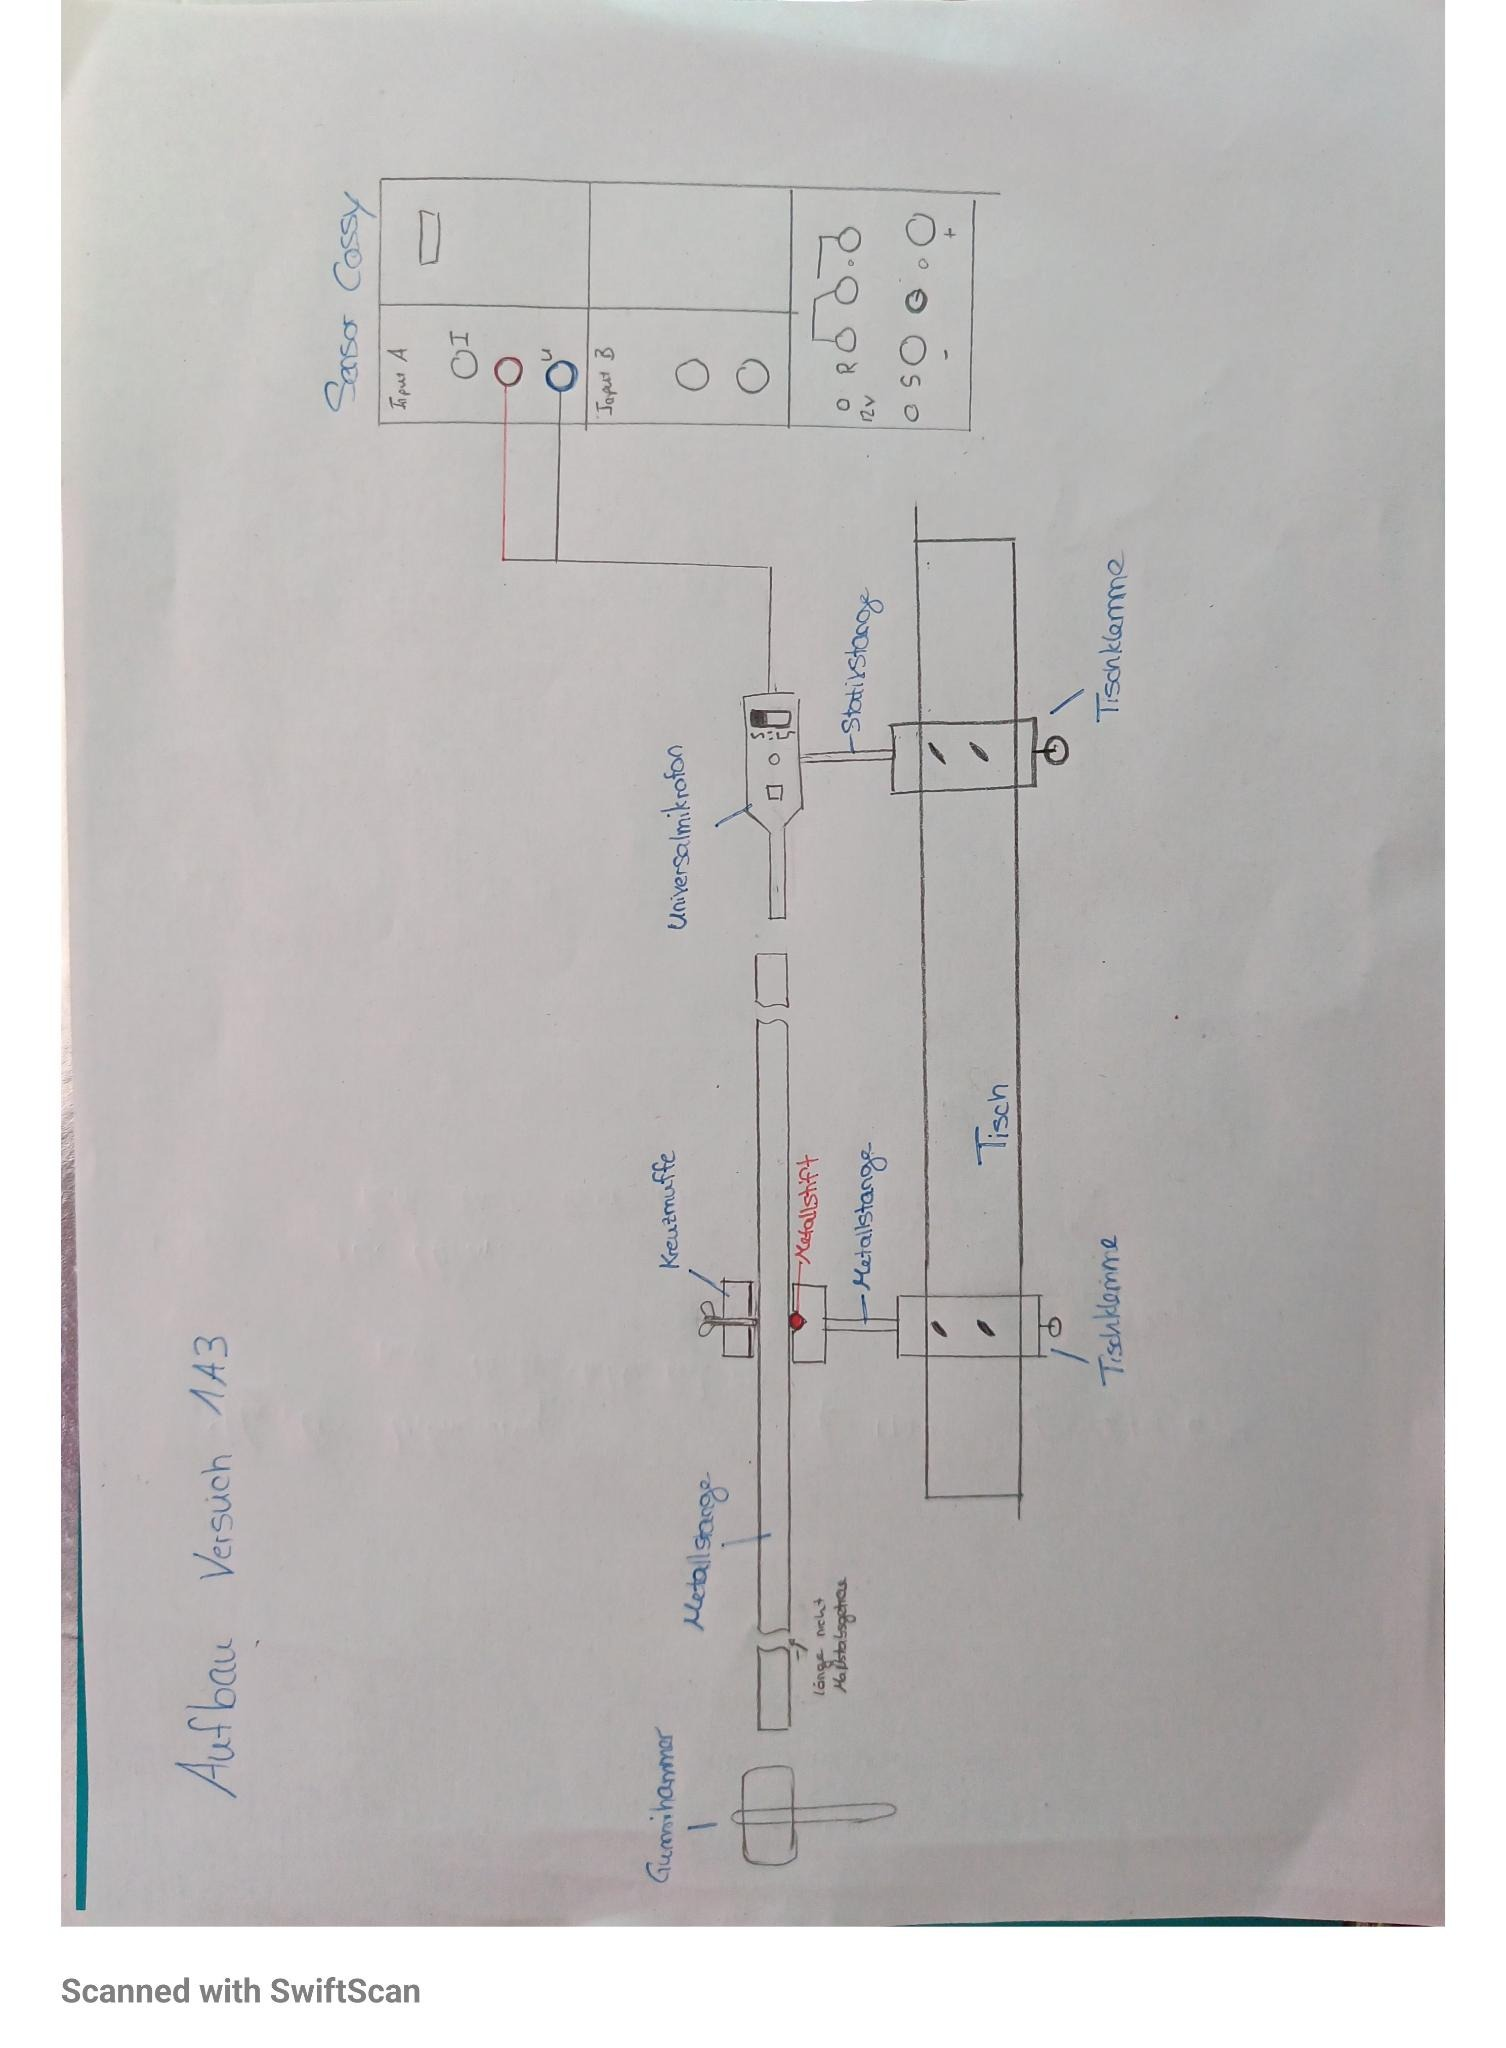
\includegraphics[width=10cm,height=10cm,keepaspectratio]{SkizzeAufbau}
Den Aufbau des experiments können sie der oben stehenden Skizze entnehmen. Hier wurden mit zwei Tischklemmen Mirkofon und halterung für den Stab  
  
  Beschreibung des Versuchsaufbaus einschließlich beschrifteter Skizze
  oder Foto. Beschreibung der Versuchsdurchführung: Handgriffe an der
  Apparatur, verwendete Messwerterfassungseinstellungen, Messbereiche,
  Triggerbedingungen, etc.
\end{aufgabe}

\begin{aufgabe}{Rohdaten}
  Stellen Sie die gemessenen Werte von $L$, $D$ und $M$ in
  tabellarischer Form dar. Visualisieren Sie einige typische
  Schwingungsverläufe sowie deren Fourierspektren in geeigneter
  Weise.
\end{aufgabe}

\begin{aufgabe}{Auswertung}
  Bestimmen Sie aus den aufgezeichneten Schwingungsvorgängen die
  Schwingungsfreqünzen und tabellieren Sie die erhaltenen
  Werte. Ermitteln Sie die Streuung der einzelnen $f_i$ und bestimmen
  Sie daraus den statistischen Fehler auf den Mittelwert. Erläutern
  und illustrieren Sie Ihr Vorgehen zur Bestimmung der systematischen
  Unsicherheiten auf die Frequenz. Diskutieren Sie die Unsicherheiten
  auf $L$, $D$ und $M$. Berechnen Sie den E-Modul und die Dichte der
  vorliegenden Stangen und die zugehörigen statistischen und
  systematischen Messunsicherheiten. Diskutieren Sie, welche
  Fehlerbeiträge den Gesamtfehler dominieren. Vergleichen Sie Ihre
  Ergebnisse mit einschlägigen Literaturwerten.
\end{aufgabe}
 
\end{document}
